\documentclass[a4paper,fleqn]{cas-dc}

\usepackage[utf8]{inputenc}
\usepackage[T1]{fontenc}
\usepackage{amsmath,amssymb,amsfonts}
\usepackage{amsthm}
\usepackage{algorithm2e}
\usepackage{booktabs}
\usepackage{graphicx}
\usepackage{multirow}
\usepackage{siunitx}
\usepackage{float}
\usepackage{xcolor}
\usepackage{url}
\usepackage{xurl}
\usepackage{tikz}
\usetikzlibrary{arrows.meta,positioning,shapes.geometric,fit,calc}
\usepackage[numbers,sort&compress]{natbib}
\usepackage{hyperref}

\hypersetup{
  colorlinks=true,
  linkcolor=blue,
  citecolor=blue,
  urlcolor=blue
}

\newtheorem{proposition}{Proposition}
\newtheorem{remark}{Remark}
\DeclareMathOperator{\Hemp}{H}
\newcommand{\tablenote}[1]{%
  \par\smallskip
  \begin{minipage}{0.98\linewidth}
  \footnotesize\textit{Note:} #1
  \end{minipage}}

\begin{document}
\let\WriteBookmarks\relax
\def\floatpagepagefraction{1}
\def\textpagefraction{.001}

\shorttitle{Limits of Fibonacci Index-Gap Coding}
\shortauthors{Ekodeck \textit{et al.}}

\title[mode=title]{Limits of Fibonacci Index-Gap Coding:
Complete Stream Costs, Compression Bounds, and Structural Controls}

\author[1,3,4]{St\'ephane Ga\"el R. EKODECK}[
    orcid=0000-0002-8094-8832]
\cormark[1]
\ead{stephane-gael.ekodeck@facsciences-uy1.cm}
\credit{Conceptualization, methodology, software, formal analysis, investigation, data curation, visualization, writing -- original draft, writing -- review and editing, supervision, project administration}

\author[1,2]{Herv\'e Tal\'e KALACHI}[
    orcid=0000-0002-2590-4159]
\ead{herve.tale@univ-yaounde1.cm}
\credit{Methodology, formal analysis, validation, writing -- review and editing}

\author[1,3,4]{Serge Alain EB\'EL\'E}[
    orcid=0000-0001-7036-7068]
\credit{Conceptualization, methodology, formal analysis, validation, writing -- review and editing}

\author[1]{Norbert DJONG WANG}
\ead{djongwangnorbert@gmail.com}
\credit{Investigation, resources, data curation, validation, writing -- review and editing}

\author[1,2]{Chantal Marguerite MVEH-ABIA}
\ead{cmmveh@yahoo.fr}
\credit{Methodology, validation, supervision, project administration, writing -- review and editing}

\affiliation[1]{
    organization={LIRIMA, TEAM GRIMCAPE, University of Yaounde I},
    city={Yaounde},
    country={Cameroon}
}

\affiliation[2]{
    organization={National Advanced School of Engineering (Polytechnic), University of Yaounde I},
    city={Yaounde},
    postcode={8390},
    country={Cameroon}
}

\affiliation[3]{
    organization={IRD, UMI, UMMISCO, IRD France Nord},
    city={Bondy},
    postcode={93143},
    country={France}
}

\affiliation[4]{
    organization={Sorbonne Universites, Univ. Paris 06, UMI 209, UMMISCO},
    city={Paris},
    postcode={75005},
    country={France}
}

\cortext[1]{Corresponding author}

\begin{abstract}
Fibonacci index gaps can look shorter than direct binary integers while still
producing a larger decodable stream. We examine where that discrepancy comes
from. The test format, Fibonacci Index-gap Shared Alphabet (FISA) 1.0, maps
each block to gaps between its Zeckendorf indices, shares one alphabet across
the file, and falls back to raw storage when needed. Its serialized size
includes the alphabet, mode and length fields, block records, and padding. The
gap map is bijective, and an exact inequality states when the shared stream is
shorter than the raw alternative. Enumerating every integer through $10^7$
gives an optimistic favorable fraction of 40.18\%, but this comparison omits
framing. On complete files, block size materially changes the outcome:
Canterbury reaches its best tested FISA ratio at 32 bytes (0.9215), whereas
Silesia reaches 0.9878 at 256 bytes. Only one Canterbury file and at most two
Silesia files compress at any tested size. At 256 bytes, just 3.70\% and
1.94\% of blocks satisfy the sufficient bound. Asymptotic term-count scaling
predicts about 815 Zeckendorf terms for a generic 2048-bit integer, versus
measured thresholds of 326--392; none of 5,000 sampled 2048-bit integers meets
either threshold. Simpler controls are smaller
after their own block-size sweeps: zero trimming reaches 0.8942 on Canterbury
and a zero-block bitmap reaches 0.9774 on Silesia. Ordinary binary set-bit gaps also dominate the optimistic
integer comparison, and established codecs win all 11 Canterbury and all 12
Silesia file comparisons. These results delimit, rather than promote, the
Fibonacci construction: the observed savings arise mainly from positional
sparsity and zero structure, not from the number system alone.
\end{abstract}

\begin{highlights}
\item FISA 1.0 serializes every field required to reconstruct the input.
\item An exact inequality identifies when its shared stream beats raw storage.
\item Generic 2048-bit integers average about 816 terms, above the 326--392 thresholds.
\item Complete-stream ratios range from 0.9215 to 0.9878 at the best tested sizes.
\item Binary-position and zero-structure controls explain the measured savings.
\item Established codecs win every paired comparison on Canterbury and Silesia.
\end{highlights}

\begin{keywords}
Lossless compression \sep Fibonacci coding \sep Zeckendorf representation
\sep Integer codes \sep Transform coding \sep Reproducible evaluation
\end{keywords}

\maketitle

\section{Introduction}
\label{sec:introduction}

Consider a transform that turns a byte block into a shorter list of integers.
That list is not yet a compressed file. The decoder still needs boundaries,
lengths, selectors, and often a model. In our experiments, those bytes decide
the result. We use ``complete cost'' for every byte inside the serialized
stream boundary. The reusable decoder, its working memory, and execution time
are measured separately.

We examine one concrete transform. Zeckendorf decomposition writes an integer
as a unique sum of non-consecutive Fibonacci terms
\cite{Zeckendorf1972}. Replacing the selected indices by adjacent differences
gives an invertible gap sequence. FISA, the Fibonacci Index-gap Shared
Alphabet format, stores these gaps with one alphabet for the file. The format
is byte-exact: it preserves leading zeros, records every length needed by the
decoder, and rejects malformed input.

The first question was simple: does the short gap sequence survive
serialization? We derived an exact stream-gain condition and a sufficient
bound on the number of selected terms. We then enumerated integers through
$10^7$ and ran complete-corpus tests at five block sizes. The integer count
looked promising. The file results did not. Only a few files compressed, and
the best block size changed with the corpus.

That mismatch led to a second question. Was Fibonacci responsible for the
small gains? We repeated the optimistic comparison with Lucas indices and
ordinary binary set-bit positions. We also built two direct zero-structure
controls. Binary positions produced shorter gap lists for most tested
integers, while zero trimming and a zero-block bitmap beat FISA on the
favorable corpora. We use FISA as a documented test case for
complete stream accounting, not as a replacement for established codecs.

The remainder of the paper is organized as follows. Section
\ref{sec:related} discusses related coding approaches. Section
\ref{sec:preliminaries} establishes the mathematical notation and worked
examples. Section \ref{sec:method} defines the transform and stream. Section
\ref{sec:analysis} gives correctness and complexity results. Section
\ref{sec:protocol} describes the experimental protocol. Section
\ref{sec:results} reports the compression evaluation. Section
\ref{sec:discussion} discusses scope and limitations.

\section{Related work}
\label{sec:related}

\subsection{Entropy and general-purpose coding}

Huffman coding remains a standard reference for symbol coding with
integer-length codewords \cite{Moffat2019Huffman}; standard treatments place
such codes within statistical, dictionary, and context modelling
\cite{Bell1990Text,Witten1999Managing}. Transform coding can preserve
information while exposing a representation better matched to a subsequent
model, as in block sorting \cite{Burrows1994BWT,Fenwick1996BWT}. Zstandard
illustrates the practical importance of jointly considering ratio, framing,
and speed \cite{Collet2021RFC8878}, while current work on Lempel--Ziv parsing
continues to improve construction and representation methods
\cite{Ellert2023LZ}.
Asymmetric numeral systems provide a finite-state alternative to Huffman and
arithmetic coding \cite{Duda2015ANS}. Zstandard uses finite-state entropy
tables for sequence symbols \cite{Collet2021RFC8878}. Such a coder could
replace FISA's fixed-width identifiers, but it would still have to serialize
the gap alphabet, frequency model, block records, and final state.
These methods learn or estimate symbol regularities across a sequence, whereas
the positional transform considered here first maps each byte block to a
single large integer.

\subsection{Fibonacci and integer representations}

Fibonacci universal codes represent positive integers with a terminator and
are useful where self-synchronization and direct integer decoding matter.
The underlying unique non-consecutive representation is due to Zeckendorf
\cite{Zeckendorf1972}, and robust complete Fibonacci code families were
studied by Fraenkel and Klein \cite{Klein1996Fibonacci}.
Practical indexing studies compare their space and decoding behavior with
other universal codes \cite{Brisaboa2021Fibonacci}. Recent work continues to
compare schemes for natural-number sequences, including Fibonacci,
Elias-family, and related representations
\cite{Elias1975,Shapira2023Natural}. Generalized
Fibonacci number systems have also been studied beyond one-dimensional integer
coding \cite{Pooksombat2022Multidim}. Domain-specific lossless compressors
provide a separate reference point: Gorilla exploits XOR structure in
floating-point time series \cite{Pelkonen2015Gorilla}, while Chimp improves
reference selection and significant-bit coding \cite{Liakos2022Chimp};
Sprintz provides a domain-specific reference point for predictive coding on
resource-constrained IoT streams; it is used for positioning rather than as an
experimental baseline \cite{Blalock2018SPRINTZ}.

The proposed representation is not a conventional Fibonacci universal code.
It first obtains the indices of the Fibonacci terms in a block integer and
then codes differences between adjacent indices. This places the method closer
to gap coding used in compressed indexes, where the distribution of
differences determines whether a universal or entropy code is effective.

\subsection{Positioning relative to the evaluated state of the art}

Table~\ref{tab:sota} distinguishes the coding role of each family. Fibonacci
universal codes address positive integers, Huffman codes symbols under a
probability model, and Lempel--Ziv-class codecs exploit repeated
substrings. FISA 1.0 is evaluated as a blockwise front-end representation
with a complete codebook and a raw fallback.

\begin{table*}[t]
\caption{Methodological positioning relative to the evaluated state of the art.}
\label{tab:sota}
\centering
\begin{tabular}{p{2.5cm}p{2.5cm}p{3.1cm}p{3.1cm}p{3.8cm}}
\toprule
Family & Coding unit & Structure exploited & Side information & Position in this study\\
\midrule
Huffman coding \cite{Moffat2019Huffman}
& Symbols & Symbol probabilities & Tree, table, or probability model
& Reference entropy-coding layer; not replaced by the index-gap transform\\
Lempel--Ziv, LZMA, Brotli, and Zstandard
\cite{Ellert2023LZ,Pavlov2015LZMA,Alakuijala2016Brotli,Collet2021RFC8878}
& Byte strings & Repeated substrings and local matches
& Dictionary references and framing
& General-purpose reference class; zlib, LZMA, Brotli, bzip2, Zstandard, and
PPMd are measured\\
Universal integer and Fibonacci codes
\cite{Elias1975,Golomb1966,RicePlaunt1971,Brisaboa2021Fibonacci}
& Positive integers or gaps & Integer magnitude and self-delimitation
& Terminators or code boundaries
& Direct conceptual baseline; measured payload ratios exceed one on both corpora\\
FISA 1.0 (framework instance)
& Fixed byte blocks & Sparse Zeckendorf indices and repeated index gaps
& Alphabet, lengths, identifiers, and mode
& Exact conditional representation with raw fallback outside favorable blocks\\
Zero-structure baselines (this evaluation)
& Fixed byte blocks & Empty blocks or boundary zero runs
& Presence bitmap or per-block trim lengths
& Simpler controls that delimit the gain attributable to Fibonacci indices\\
\bottomrule
\end{tabular}
\tablenote{The last column contains only conclusions supported by this study.}
\end{table*}

\paragraph{Positioning statement.}
The contribution is a reversible representation layer, not a
replacement entropy coder or dictionary model. Its direct comparison targets
are universal integer codes at the transformed-stream level and mature
lossless codecs at the complete-file level.

\section{Preliminaries}
\label{sec:preliminaries}

This section establishes the mathematical objects used throughout the paper:
the Fibonacci sequence, Zeckendorf decomposition, and the gap reduction that
forms the basis of the FISA transform.

\subsection{Fibonacci sequence}

The Fibonacci sequence is defined by
\begin{equation}
F_0=0,\qquad F_1=1,\qquad F_n=F_{n-1}+F_{n-2}\quad(n\geq2).
\label{eq:fibonacci}
\end{equation}
Its closed form is
\begin{equation}
F_n=\frac{\phi^n-\psi^n}{\sqrt{5}},\qquad
\phi=\frac{1+\sqrt{5}}{2},\quad\psi=\frac{1-\sqrt{5}}{2}.
\label{eq:binet}
\end{equation}
Equation~\eqref{eq:binet} explains the growth
$F_n=\Theta(\phi^n)$, but the codec does not evaluate it numerically:
floating-point rounding cannot guarantee exact reconstruction for large
indices. Required values are generated by exact integer addition, and fast
doubling is used for random access. Algorithm~\ref{alg:fibonacci} constructs
the exact table required for greedy decomposition.

\begin{algorithm}[t]
\caption{\texttt{FibonacciTable($d$)}}
\label{alg:fibonacci}
\KwIn{Non-negative integer $d$}
\KwOut{Exact Fibonacci values covering $d$}
$V\leftarrow[0,1,1]$\;
\While{$V[-1]\leq d$}{
  append $V[-1]+V[-2]$ to $V$\;
}
\Return $V$\;
\end{algorithm}

Algorithm~\ref{alg:fibonacci} favors a self-contained specification. The
compiled implementation caches the generated table across blocks.

For example, $F_{10}=55$ and $F_{20}=6765$. The index grows linearly while
the represented value grows exponentially. This motivates representing
selected terms by indices rather than by their values.

\subsection{Notation}

Table~\ref{tab:notation} summarizes the symbols used in the transform and its
analysis.

\begin{table}[t]
\caption{Main notation.}
\label{tab:notation}
\centering
\begin{tabular}{ll}
\toprule
Symbol & Meaning\\
\midrule
$m$ & Input byte message or block\\
$d$ & Non-negative block integer\\
$F_i$ & Fibonacci value with index $i$\\
$I$ & Descending Zeckendorf indices\\
$t=|I|$ & Number of selected Zeckendorf terms\\
$G$ & Reduced index-gap sequence\\
$\mathcal{A}$ & Ordered alphabet of distinct gaps\\
$S$ & Alphabet-identifier sequence\\
$w$ & Identifier width\\
$x\Vert y$ & Concatenation\\
$|x|$ & Length in the stated unit\\
\bottomrule
\end{tabular}
\end{table}

Table~\ref{tab:acronyms} gives the abbreviations retained in the remainder of
the paper.

\begin{table}[t]
\caption{Abbreviations used in the method and experiments.}
\label{tab:acronyms}
\centering
\begin{tabular}{ll}
\toprule
Abbreviation & Expansion\\
\midrule
FISA & Fibonacci Index-gap Shared Alphabet\\
FIPB & Fibonacci Independent Per-Block baseline\\
RLE & Run-length encoding\\
LEB128 & Little-Endian Base-128 integer encoding\\
\bottomrule
\end{tabular}
\end{table}

\subsection{Integer decomposition via Fibonacci indices}

\subsubsection{Basic term decomposition}

Greedy decomposition repeatedly selects the largest Fibonacci value not
exceeding the current remainder. For $d=18324$,
\begin{equation}
18324=F_{22}+F_{15}+F_4=17711+610+3.
\end{equation}
The direct binary representation requires 15 bits. Writing the selected
Fibonacci values separately requires the optimistic sum $15+10+2=27$ bits,
before delimiters, so this example expands.

\subsubsection{Term indices}

The same decomposition has index sequence $I=[22,15,4]$. The optimistic sum
of index bit lengths is $5+4+3=12$ bits. This motivates index storage, but it
is not yet a complete code because element boundaries remain unspecified.

\subsubsection{Reduced term indices}

Taking adjacent differences gives
\begin{equation}
G=[22-15,15-4,4]=[7,11,4].
\end{equation}
The optimistic bit-length sum is $3+4+3=10$ bits. Thus the example follows
$15>12>10$ at the representation level. The complete codec subsequently
counts the alphabet, widths, lengths, padding, and framing omitted here.
Algorithm~\ref{alg:decompose} formalizes the decomposition and adjacent-gap
reduction.

\begin{algorithm}[t]
\caption{\texttt{DecomposeAndReduce($d$)}}
\label{alg:decompose}
\KwIn{Non-negative integer $d$}
\KwOut{Reduced gaps $G$}
$I\leftarrow[]$; $V\leftarrow\texttt{FibonacciTable}(d)$\;
\While{$d>0$}{
  choose largest $i$ such that $V[i]\leq d$\;
  append $i$ to $I$; $d\leftarrow d-V[i]$\;
}
\For{$j\leftarrow0$ \KwTo $|I|-2$}{
  $G[j]\leftarrow I[j]-I[j+1]$\;
}
\If{$|I|>0$}{$G[|I|-1]\leftarrow I[|I|-1]$\;}
\Return $G$\;
\end{algorithm}

\subsection{Alphabet extraction and binary transformation}

For
\[
G=[150,200,150,300,200,250,300,150,200],
\]
the frequencies of 150, 200, 300, and 250 are 3, 3, 2, and 1. Sorting by
decreasing frequency and then first occurrence gives
\[
\mathcal{A}=[150,200,300,250],\quad
S=[0,1,0,2,1,3,2,0,1].
\]
Since $|\mathcal{A}|=4$, identifiers use $w=2$ bits. The packed stream is
\[
00\Vert01\Vert00\Vert10\Vert01\Vert11\Vert10\Vert00\Vert01.
\]
Fixed width makes symbol boundaries unambiguous. The alphabet and its length
are included in the payload. Algorithm~\ref{alg:alphabet} gives the
frequency-ordered alphabet construction used by the reference implementation.

\begin{algorithm}[t]
\caption{\texttt{ExtractAlphabet($G$)}}
\label{alg:alphabet}
\KwIn{Gap sequence $G$}
\KwOut{$\mathcal{A}$, identifiers $S$, width $w$}
count values and record first positions\;
$\mathcal{A}\leftarrow$ values sorted by decreasing count, then first position\;
replace each $G[j]$ by its index $S[j]$ in $\mathcal{A}$\;
$w\leftarrow\lceil\log_2|\mathcal{A}|\rceil$ if $\mathcal{A}\neq\varnothing$, else $0$\;
\Return $(\mathcal{A},S,w)$\;
\end{algorithm}

\section{FISA 1.0 test format}
\label{sec:method}

\subsection{Encoding pipeline}

FISA is specified here to make the accounting experiment reproducible. It is
not introduced as a competitor to general-purpose codecs.
Figure~\ref{fig:pipeline} presents the complete pipeline. The transform first
produces an exact candidate payload. The selector then compares complete
serialized lengths and stores either the Fibonacci payload or the raw block.

\begin{figure*}[t]
\centering
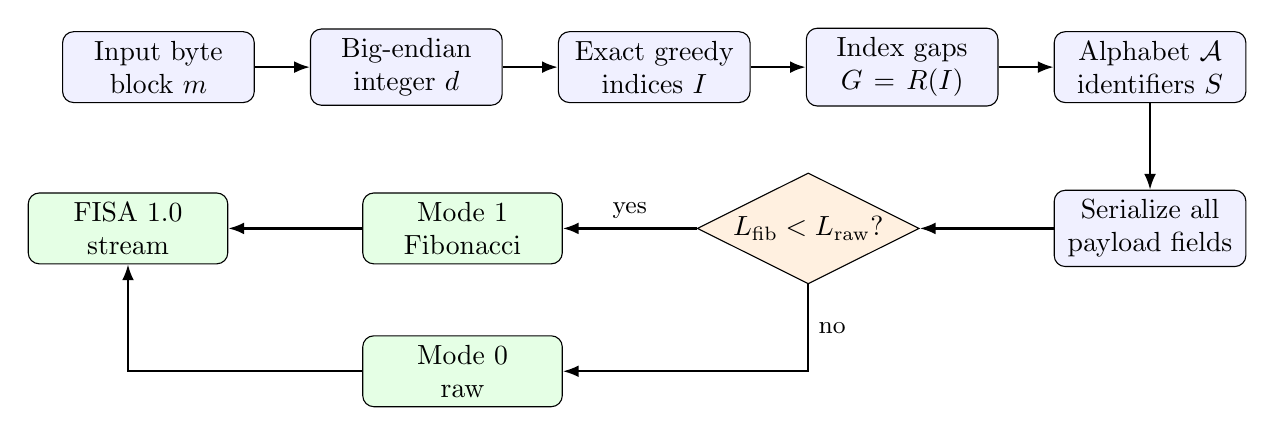
\begin{tikzpicture}[
  node distance=7mm and 7mm,
  box/.style={draw, rounded corners, align=center, minimum height=9mm,
              text width=22mm, fill=blue!6},
  decision/.style={draw, diamond, aspect=2.0, align=center, fill=orange!12,
                   inner sep=1.5pt},
  arrow/.style={-{Latex[length=2mm]}, thick},
  output/.style={draw, rounded corners, align=center, minimum height=9mm,
                 text width=23mm, fill=green!10}
]
\node[box] (input) {Input byte\\block $m$};
\node[box, right=of input] (integer) {Big-endian\\integer $d$};
\node[box, right=of integer] (decomp) {Exact greedy\\indices $I$};
\node[box, right=of decomp] (gaps) {Index gaps\\$G=R(I)$};
\node[box, right=of gaps] (alphabet) {Alphabet $\mathcal{A}$\\identifiers $S$};
\node[box, below=11mm of alphabet] (serialize) {Serialize all\\payload fields};
\node[decision, left=17mm of serialize] (select) {$L_{\rm fib}<L_{\rm raw}$?};
\node[output, left=17mm of select] (fib) {Mode 1\\Fibonacci};
\node[output, below=9mm of fib] (raw) {Mode 0\\raw};
\node[output, left=17mm of fib] (container) {FISA 1.0\\stream};
\draw[arrow] (input)--(integer);
\draw[arrow] (integer)--(decomp);
\draw[arrow] (decomp)--(gaps);
\draw[arrow] (gaps)--(alphabet);
\draw[arrow] (alphabet)--(serialize);
\draw[arrow] (serialize)--(select);
\draw[arrow] (select)--node[above,font=\small]{yes}(fib);
\draw[arrow] (select.south)|-node[pos=0.25,right,font=\small]{no}(raw.east);
\draw[arrow] (fib)--(container);
\draw[arrow] (raw.west)-|(container.south);
\end{tikzpicture}
\caption{Blockwise encoding pipeline. All information needed by the decoder is
serialized before the mode decision.}
\label{fig:pipeline}
\end{figure*}

\subsection{Exact decomposition}

Let $(F_n)_{n\geq 0}$ be the Fibonacci sequence,
\begin{equation}
F_0=0,\qquad F_1=1,\qquad F_n=F_{n-1}+F_{n-2}.
\end{equation}
We use the conventional positive terms $F_2=1,F_3=2,\ldots$. For a
non-negative block integer $d$, the greedy decomposition returns a descending
sequence
\begin{equation}
I(d)=(i_0,i_1,\ldots,i_{t-1}), \qquad i_j-i_{j+1}\geq 2,
\end{equation}
such that
\begin{equation}
d=\sum_{j=0}^{t-1}F_{i_j}.
\label{eq:zeckendorf}
\end{equation}
For $d=0$, the index sequence is empty. The implementation uses exact integer
arithmetic and builds Fibonacci values iteratively until the block value is
covered.

\subsection{Index-gap transform}

For a non-empty index sequence $I$, define
\begin{equation}
R(I)=G=(g_0,\ldots,g_{t-1}),
\end{equation}
where
\begin{equation}
g_j=i_j-i_{j+1}\quad(0\leq j<t-1),\qquad
g_{t-1}=i_{t-1}.
\label{eq:gaps}
\end{equation}
The inverse is a suffix sum:
\begin{equation}
i_{t-1}=g_{t-1},\qquad
i_j=g_j+i_{j+1}.
\label{eq:inverse}
\end{equation}
The gap values are frequently much smaller than the original indices. The
representation builds an alphabet $\mathcal{A}$ from the distinct values in
$G$, ordered by decreasing frequency with first occurrence as the tie-breaker.
Each gap is replaced by its zero-based identifier in $\mathcal{A}$.

\subsection{Independent per-block payload (FIPB baseline)}
\label{sec:fipb-payload}

The independent per-block baseline, denoted FIPB, serializes a complete local
Fibonacci payload for each block. It contains:
\begin{enumerate}
\item the alphabet size as an unsigned LEB128 integer;
\item the number of symbols as an unsigned LEB128 integer;
\item one byte for the fixed symbol width;
\item every alphabet value as an unsigned LEB128 integer;
\item the packed-stream length as an unsigned LEB128 integer; and
\item fixed-width identifiers packed most-significant bit first.
\end{enumerate}
Padding bits in the final byte are zero and are included in the measured size.
This explicit baseline prevents the evaluation from treating the local
alphabet or delimiters as free information. FISA 1.0, defined next, instead
amortizes one alphabet over the complete stream and does not repeat it inside
each transformed block.

\subsection{Shared-alphabet stream}
\label{sec:shared-alphabet}

Because repeating an alphabet in every block creates substantial overhead,
FISA 1.0 constructs one frequency-ordered gap
alphabet for all blocks in a stream. Each transformed block then stores only its
symbol count, packed length, and identifiers. Local mode selection retains a
block only when this reduced payload is shorter than the raw block. A second
stream-level decision compares the complete shared-alphabet stream with a raw
stream, including the global alphabet and all framing:
\begin{equation}
L_{\mathrm{FISA\,1.0}}(x)=
\min\{L_{\mathrm{shared}}(x),L_{\mathrm{raw-stream}}(x)\}.
\label{eq:shared-selector}
\end{equation}
Both branches are decoded and verified byte-for-byte in the experiments.

\begin{proposition}[Exact amortized gain condition]
\label{prop:amortized-gain}
Let $N=\sum_i n_i$ be the input length, $B$ the number of blocks,
$\beta$ the nominal block size,
$a=|\mathcal{A}|$, $w=\lceil\log_2 a\rceil$, and $u(z)$ the byte length of unsigned
LEB128. If block $i$ contains $k_i$ gap symbols, define
$q_i=\lceil k_iw/8\rceil$, $p_i=u(k_i)+u(q_i)+q_i$, and
$s_i=\min\{n_i,p_i\}$. The complete shared representation is shorter than the
raw stream if and only if
\begin{equation}
\begin{aligned}
&u(\beta)+u(B)+u(a)+1+\sum_{g\in\mathcal{A}}u(g)\\
&\quad+\sum_{i=1}^{B}\left[1+u(n_i)+u(s_i)+s_i\right] < N,
\end{aligned}
\label{eq:exact-shared-condition}
\end{equation}
\end{proposition}

\begin{proof}
The terms in Eq.~\eqref{eq:exact-shared-condition} are respectively the
global block-size, block-count, alphabet-size and width fields, serialized
alphabet values, and complete block records. The magic, format identifier,
stream mode, and original-length field occur in both candidates and cancel.
The remaining inequality is exactly
$L_{\mathrm{shared}}<L_{\mathrm{raw-stream}}$.
\end{proof}

Under equal amortization of the global metadata
$C_A=u(\beta)+u(B)+u(a)+1+\sum_{g\in\mathcal{A}}u(g)$, a computable sufficient threshold is
\begin{equation}
k^\star=\max\left\{k:
1+u(n)+u(p(k))+p(k)+\left\lceil C_A/B\right\rceil<n\right\},
\label{eq:k-threshold}
\end{equation}
with $p(k)=u(k)+u(\lceil kw/8\rceil)+\lceil kw/8\rceil$. Thus a term-count
criterion is meaningful only when identifier width and amortized alphabet
cost are also specified.

\paragraph{Stream bounds and a constructive best case.}
The raw fallback gives, for every non-empty input of $N$ bytes,
\begin{equation}
\frac{6+u(N)}{N}\leq \rho_{\rm FISA}
\leq 1+\frac{6+u(N)}{N}.
\label{eq:fisa-universal-bounds}
\end{equation}
The lower inequality counts only the mandatory outer fields; it is not
generally attainable. The upper inequality follows by selecting the raw
candidate. For an all-zero input whose length is an exact multiple of
$\beta$, the shared alphabet is empty and the transformed length is
\begin{equation}
6+u(N)+u(\beta)+u(N/\beta)+2+
\frac{N}{\beta}\left(4+u(\beta)\right).
\label{eq:zero-stream-cost}
\end{equation}
At $N=1$\,MiB and $\beta=256$, Eq.~\eqref{eq:zero-stream-cost} gives a ratio
of 0.02345. Hence there is no universal lower bound near 0.80: the useful
class consists of highly structured inputs, although simpler zero controls
encode that class more effectively in the corpus experiments.

\subsection{FISA 1.0 stream and fallback}

The stream begins with the four-byte magic value \texttt{FISA}, a one-byte
format identifier with value 1, a stream-mode byte, and the original byte
length. Raw-stream mode stores the original bytes directly. Shared mode then
stores the nominal block size, block count, global gap alphabet, and identifier
width. Each block stores a mode byte, original block length, payload length,
and payload. Mode 0 stores raw bytes; mode 1 stores shared-alphabet identifiers.

For comparison, the independent FIPB baseline chooses the mode of a block
$x$ according to
\begin{equation}
\operatorname{mode}(x)=
\begin{cases}
\mathrm{FIB},&L_{\mathrm{fib}}(x)<L_{\mathrm{raw}}(x),\\
\mathrm{RAW},&\text{otherwise},
\end{cases}
\label{eq:selector}
\end{equation}
where both lengths are known exactly after serialization. The strict
inequality avoids choosing the more complex representation on a tie.
Within a FISA shared stream, the analogous local decision compares the
shared-identifier body $p_i$ with the raw block, without charging a local
alphabet; the global alphabet and complete framing are then handled by
Proposition~\ref{prop:amortized-gain}.

\begin{proposition}[Independent per-block gain condition]
\label{prop:gain}
For a block $x$ in the FIPB baseline, Fibonacci mode is selected if and only
if the independently serialized payload, including its local alphabet,
lengths, symbol width, packed identifiers, and padding, occupies fewer bytes
than $x$. The selected FIPB block payload never exceeds the
corresponding raw payload. This proposition concerns the independent
per-block selector in Eq.~\eqref{eq:selector}; the complete FISA shared-stream
condition is Proposition~\ref{prop:amortized-gain}.
\end{proposition}

\begin{proof}
All Fibonacci fields are materialized before the comparison in
Eq.~\eqref{eq:selector}. The encoder returns that payload only under the strict
inequality $L_{\mathrm{fib}}(x)<L_{\mathrm{raw}}(x)$; otherwise it returns
$x$. The selected payload length is
$\min\{L_{\mathrm{fib}}(x),L_{\mathrm{raw}}(x)\}$.
\end{proof}

Algorithm~\ref{alg:encode} implements this independent FIPB block selector.

\begin{algorithm}[t]
\caption{Hybrid FIPB encoding of one independent block}
\label{alg:encode}
\KwIn{Byte block $x$}
\KwOut{Mode and payload}
$d\leftarrow\operatorname{IntegerFromBytes}(x)$\;
$I\leftarrow\operatorname{GreedyFibonacciIndices}(d)$\;
$G\leftarrow R(I)$\;
$(\mathcal{A},S)\leftarrow\operatorname{Alphabetize}(G)$\;
$p\leftarrow\operatorname{Serialize}(\mathcal{A},S)$\;
\eIf{$|p|<|x|$}{
  \Return $(\mathrm{FIB},p)$\;
}{
  \Return $(\mathrm{RAW},x)$\;
}
\end{algorithm}

\subsection{Decoding processes}

The FIPB decoder reverses the independent per-block mode. A raw block is
copied directly. For a Fibonacci block, it parses the local alphabet and
packed identifiers, reconstructs $G$, lifts suffix sums to recover $I$, and
evaluates Eq.~\eqref{eq:zeckendorf}. The declared block length restores
leading zero bytes. The FISA decoder performs the same inverse operations but
parses the stream-level alphabet once and uses it for every shared-mode block.
Algorithm~\ref{alg:decode} specifies the inverse FIPB block operation; FISA
uses the same suffix-sum and Fibonacci reconstruction with the shared
alphabet supplied by the stream header.

\begin{algorithm}[t]
\caption{\texttt{DecodeFIPBBlock(mode,payload,$\ell$)}}
\label{alg:decode}
\KwIn{Mode, payload, declared byte length $\ell$}
\KwOut{Original block}
\If{mode is RAW}{\Return payload\;}
parse $(\mathcal{A},|S|,w,S)$ from payload\;
$G[j]\leftarrow\mathcal{A}[S[j]]$ for every identifier\;
$I[|G|-1]\leftarrow G[|G|-1]$\;
\For{$j\leftarrow |G|-2,|G|-3,\ldots,0$}{
  $I[j]\leftarrow G[j]+I[j+1]$\;
}
$d\leftarrow\sum_j F_{I[j]}$\;
\Return $d$ as exactly $\ell$ big-endian bytes\;
\end{algorithm}

\section{Correctness and analytical properties}
\label{sec:analysis}

This section checks the properties required by the format: bijectivity of the
gap map, lossless reconstruction, the entropy consequences of a bijection,
and computational complexity.

\begin{proposition}[Bijectivity of index-gap reduction]
For every finite descending integer sequence $I$, the map $R$ defined in
Eq.~\eqref{eq:gaps} is bijective.
\end{proposition}

\begin{proof}
Equation \eqref{eq:inverse} reconstructs the final index directly and every
preceding index recursively. Hence each gap vector has at most one preimage.
Substituting Eq.~\eqref{eq:inverse} into Eq.~\eqref{eq:gaps} recovers every
component of $G$, establishing existence and uniqueness.
\end{proof}

\begin{proposition}[Lossless block reconstruction]
Given a valid payload and the original block length, the decoder reconstructs
the unique input block.
\end{proposition}

\begin{proof}
The serialized alphabet maps each valid symbol identifier to one gap. The
inverse transform reconstructs the unique index sequence. Summation of the
exact Fibonacci terms in Eq.~\eqref{eq:zeckendorf} reconstructs $d$. Conversion
to the declared byte length restores leading zero bytes. The decoder rejects
invalid identifiers, inconsistent lengths, truncated payloads, values that do
not fit the declared block length, and trailing bytes.
\end{proof}

\subsection{Entropy interpretation}

Let $X$ be a discrete random variable and $R$ a bijection. Then
$\Hemp(R(X))=\Hemp(X)$ because $R$ only relabels outcomes and preserves their
probabilities. For a block process $(X_t)$, componentwise invertibility also
preserves every joint entropy
$\Hemp(R(X_1),\ldots,R(X_T))=\Hemp(X_1,\ldots,X_T)$ and preserves
the entropy rate when the limit exists. It need not preserve the redundancy
of a restricted coding model: symbol marginals, apparent empirical order, and
factorization costs can change after transformation. Compression can improve
when the transformed sequence is better matched by the
chosen finite-context or alphabet code, without any reduction in source
entropy. The empirical zero-order byte entropy reported here is
descriptive rather than a universal finite-file lower bound.

\subsection{Expected Zeckendorf term count}
\label{sec:expected-terms}

Lekkerkerker's theorem states that the average number of summands for
integers in $[F_n,F_{n+1})$ is \cite{Kologlu2011Summands}
\begin{equation}
\mathbb{E}[t\mid F_n\leq d<F_{n+1}]
=\frac{n}{\varphi^2+1}+O(1),
\label{eq:lekkerkerker}
\end{equation}
where $\varphi=(1+\sqrt{5})/2$. Since
$F_n=\varphi^n/\sqrt{5}+O(\varphi^{-n})$, a generic $\ell$-bit integer has
\begin{equation}
\mathbb{E}[t]
=\frac{\ell}{(\varphi^2+1)\log_2\varphi}+O(1)
\approx 0.3981\,\ell+O(1).
\label{eq:expected-terms}
\end{equation}
This scaling predicts about 815 terms for a 2048-bit integer. It does not by
itself determine complete stream size, but it provides a source-independent
reference for the empirical threshold in Eq.~\eqref{eq:k-threshold}.

\subsection{Complexity}

Let $\ell_d$ be the bit length of the block integer, $t$ the number of selected
Fibonacci terms, and $k$ the number of distinct gaps. Exact fast doubling
computes a Fibonacci term in $O(M(\ell_d)\log n)$ bit operations, where
$M(\ell_d)$ is
the multiplication cost. The reference greedy method builds the required
Fibonacci values once and performs at most $O(\ell_d)$ term selections because
the largest index is $\Theta(\ell_d)$ and selected indices are non-consecutive. Gap
construction is $O(t)$. Alphabet counting is expected $O(t)$, followed by
$O(k\log k)$ ordering. The representation requires $O(\ell_d+t)$ bits, excluding
interpreter overhead. In the measured implementation, decomposition dominates
encoding time; decoding is cheaper when the raw-stream branch is selected.

\section{Experimental protocol}
\label{sec:protocol}

The experiments below test the representation, its cost model, and the
alternative explanations introduced in Section~\ref{sec:related}.

\subsection{Research questions}

The experiments address five questions:
\begin{description}
\item[RQ1] For which integers does the gap representation reduce the
optimistic bit count?
\item[RQ2] Which components determine the complete serialized size?
\item[RQ3] How does the hybrid representation compare with raw storage,
universal integer codes, and established lossless codecs?
\item[RQ4] Is the measured effect specific to Fibonacci, or explained more
simply by positional or zero-block structure?
\item[RQ5] How sensitive is the complete shared stream to block size?
\end{description}

\subsection{Data}

The synthetic corpus contains seven deterministic 64\,KiB files generated
with seed 20260608: zeros, ones, alternating bytes, a low-alphabet sequence,
periodic text, a byte ramp, and pseudorandom bytes. Canterbury contains all 11
files in the standard archive. Silesia contains 12 heterogeneous files.
Python sensitivity experiments use fixed 64\,KiB prefixes; these results are
labelled as ablations and are not used for full-corpus claims. The compiled
FISA implementation evaluates every complete Silesia file.
The 100,000,000-byte enwik8 file is evaluated by both FISA and the
general-purpose baselines. Five deterministic monotone sequences
of 100,000 integers cover dense, geometric, posting-like, and quadratic
growth regimes.
The term-count scaling check draws 5,000 uniformly sampled integers at each
exact bit length from 128 to 2048, using seed 20260610. A separate byte-order
check reverses each 256-byte block before encoding and after decoding; it uses
Canterbury and the fixed Silesia prefixes.

The archive SHA-256 digests are recorded in the experiment manifest and are
verified by the reproducibility scripts before corpus extraction.

\subsection{Configurations and metrics}

The independent per-block baseline is evaluated with block sizes of 16, 64,
256, and 512 bytes. The compiled shared-stream implementation evaluates the
complete Canterbury and Silesia corpora at 16, 32, 64, 128, and 256 bytes.
The 256-byte setting remains the common reference for comparisons that require
one fixed block size. The baselines
are raw storage, byte RLE, zlib level 9, bzip2
level 9, LZMA preset 9~\cite{Pavlov2015LZMA}, Brotli quality 11
\cite{Alakuijala2016Brotli}, Zstandard level 19, and PPMd order 6.
Universal-code measurements include Elias gamma and delta
\cite{Elias1975}, Fibonacci universal coding, unsigned LEB128, and an oracle
Rice parameter \cite{Golomb1966,RicePlaunt1971}. These universal-code values
are payload-only and remain optimistic. Additional complete comparisons
use canonical Huffman, signalled Rice, a stream-level shared alphabet, and
Elias--Fano on monotone sequences.

The primary metric is
\begin{equation}
\rho=\frac{\text{serialized bytes}}{\text{input bytes}}.
\end{equation}
We also record bits per byte, execution time, peak Python allocation, and
empirical zero- and first-order conditional entropy. Every FISA output is
decoded and compared byte-for-byte with the input. The implementation is
tested over all integers from 1 to 9999, arbitrary byte strings, leading
zeros, multiple block sizes, and malformed streams.

\subsection{Paired comparison}

Per-file comparison uses the complete shared-alphabet stream and the smallest
modern baseline on the same file. Canterbury contributes 11 pairs and Silesia
12. We report win counts and median size factors. This finite-corpus summary
does not treat files as a random sample from a wider population. Fixed-prefix
measurements are used only for exploratory ablations.

\subsection{AI-assisted tooling and verification}

The OpenAI Codex coding agent assisted with source-code editing, experiment orchestration,
language editing, and manuscript-format checks. It did not supply experimental
data or replace the stated algorithms. The authors inspected the changes,
reran the deterministic workflows, verified every FISA stream by decoding it,
and checked the reported tables against the machine-readable result files.

\section{Results}
\label{sec:results}

\subsection{Integer-range viability}

Figure~\ref{fig:range-scaling} compares the direct binary length with the sum
of individual gap bit lengths for every integer from 1 through $d=10^7$.
This comparison excludes alphabets and framing and provides an upper
bound on the attainable benefit. It characterizes only this finite range,
whose largest values require about 24 bits; the much larger integers induced
by blocks of up to 256 bytes are assessed through the corpus experiments
rather than inferred from this enumeration.

\begin{figure*}[t]
\centering
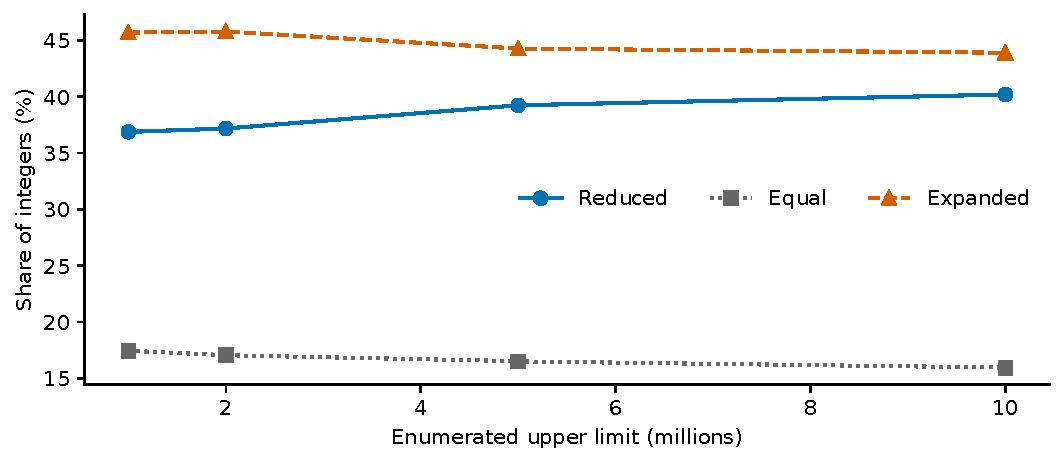
\includegraphics[width=0.72\textwidth]{artwork/Figure_2_Range_Scaling.pdf}
\caption{Integer-range scaling. Fractions of enumerated integers whose
delimiter-free Fibonacci gap length is shorter than, equal to, or longer than
the direct binary length.}
\label{fig:range-scaling}
\end{figure*}

The favorable fraction increases with the tested range and the optimistic
mean crosses zero before $10^7$. This trend concerns only gap magnitudes;
Eq.~\eqref{eq:exact-shared-condition} remains the criterion for complete
compression.

\subsection{Is the effect specific to Fibonacci?}

Table~\ref{tab:numeration} applies the same optimistic gap-bit metric to three
index systems over $1\leq d\leq10^6$. The canonical Fibonacci result is not
optimal under this metric. A greedy Lucas decomposition has a larger favorable
fraction, while set-bit positions in the ordinary binary representation are
shortest for most integers. The latter omits complete delimiters, as do the
Fibonacci and Lucas rows, and serves as a structural control rather
than a deployable codec.

\begin{table*}[t]
\caption{Optimistic index-gap comparison over $1\leq d\leq10^6$.}
\label{tab:numeration}
\centering
\begin{tabular}{lrrrrrr}
\toprule
Basis & Gain (\%) & Equal (\%) & Expansion (\%) & Mean bits & Mean terms & Unique best (\%)\\
\midrule
Fibonacci (Zeckendorf) & 36.87 & 17.46 & 45.67 & 19.0818 & 7.8945 & 5.36\\
Lucas (greedy) & 48.35 & 18.07 & 33.59 & 18.4216 & 8.1328 & 9.62\\
Binary set-bit positions & 98.39 & 1.61 & 0.00 & 15.4673 & 9.8850 & 73.67\\
\bottomrule
\end{tabular}
\tablenote{``Unique best'' is the fraction for which one method alone has the
shortest measured gap sequence.}
\end{table*}

This comparison changes the interpretation. Fibonacci provides a canonical
non-consecutive decomposition, but the gain mechanism is position-gap coding
under an amortized model. The Fibonacci basis is one exactly reversible
instance, not an empirically optimal basis.

\subsection{Empirical calibration of the term threshold}

Table~\ref{tab:kstar} calibrates Eq.~\eqref{eq:k-threshold} on complete files.
Because each file has its own alphabet and amortized metadata, $k^\star$ is a
stream-level quantity rather than one corpus-wide constant. At 256 bytes it is
390--392 terms on Canterbury and 326 terms on every Silesia file. Only 3.70\%
and 1.94\% of complete blocks satisfy the sufficient bound. These fractions
closely track the 3.75\% and 1.94\% of all blocks whose local shared payload is
actually selected.

\begin{table*}[t]
\caption{Empirical calibration of the sufficient term threshold.}
\label{tab:kstar}
\centering
\begin{tabular}{lrrrrrr}
\toprule
Corpus & Files & $k^\star$ range & Complete blocks & Bound satisfied (\%) &
All blocks & Shared selected (\%)\\
\midrule
Canterbury & 11 & 390--392 & 10,975 & 3.699 & 10,986 & 3.750\\
Silesia & 12 & 326 & 827,882 & 1.937 & 827,890 & 1.938\\
\bottomrule
\end{tabular}
\tablenote{The calibration uses complete 256-byte blocks. The selected
fraction includes final partial blocks.}
\end{table*}

The close agreement does not turn the sufficient condition into a necessary
one. It shows that, under the measured alphabet widths and low amortized
metadata, term count is the dominant local selector. It also quantifies why
the favorable regime occupies only a small minority of standard-corpus
blocks.

\subsection{Generic term-count scaling}

Table~\ref{tab:term-scaling} checks Eq.~\eqref{eq:expected-terms} using
uniformly sampled integers of exact bit length. The asymptotic prediction and
simulation agree closely. For 256-byte blocks, the simulated mean is 815.63
terms, compared with the measured complete-stream thresholds of 326 on
Silesia and 390--392 on Canterbury. None of the 5,000 sampled 2048-bit
integers meets either threshold. The corpus fractions in
Table~\ref{tab:kstar} are therefore attributable to non-generic structure,
principally zero-dominated blocks.

\begin{table*}[t]
\caption{Zeckendorf term-count scaling for uniformly sampled exact-length integers.}
\label{tab:term-scaling}
\centering
\begin{tabular}{rrrrrr}
\toprule
Block (bytes) & Bits & Asymptotic mean & Simulated mean & Std. dev. &
Simulated range\\
\midrule
16  & 128  & 50.96  & 51.41  & 4.05  & 36--65\\
32  & 256  & 101.92 & 102.17 & 5.67  & 83--122\\
64  & 512  & 203.84 & 204.28 & 8.11  & 175--238\\
128 & 1024 & 407.68 & 408.31 & 11.48 & 354--453\\
256 & 2048 & 815.35 & 815.63 & 16.36 & 748--873\\
\bottomrule
\end{tabular}
\tablenote{Each row contains 5,000 samples generated with seed 20260610.
The asymptotic column uses Eq.~\eqref{eq:expected-terms}.}
\end{table*}

\subsection{Ablation of representation costs}

Table \ref{tab:ablation} separates three quantities on Canterbury and fixed
Silesia prefixes: the bit lengths of the Fibonacci indices, the bit lengths of
the reduced gaps, and the complete
serialized payload. Gap reduction consistently improves on direct index
storage. On Canterbury with 256-byte blocks, the gap ratio is 0.9439 while the
complete payload ratio is 1.6279. The 0.6840 difference identifies the cost of
alphabet values, identifiers, lengths, width fields, and byte padding.

\begin{table*}[t]
\caption{Exploratory mean ablation ratios.}
\label{tab:ablation}
\centering
\begin{tabular}{llrrr}
\toprule
Corpus & Block (bytes) & Indices & Gaps & Payload\\
\midrule
Canterbury & 16  & 2.4250 & 0.8892 & 1.9046\\
Canterbury & 64  & 3.2478 & 0.9189 & 1.7424\\
Canterbury & 256 & 4.1008 & 0.9439 & 1.6279\\
Canterbury & 512 & 4.5120 & 0.9496 & 1.6377\\
Silesia sample & 16  & 2.4771 & 0.9024 & 1.9354\\
Silesia sample & 64  & 3.2404 & 0.9151 & 1.7347\\
Silesia sample & 256 & 4.0288 & 0.9252 & 1.5955\\
Silesia sample & 512 & 4.5015 & 0.9452 & 1.6370\\
\bottomrule
\end{tabular}
\tablenote{The Silesia measurements use fixed 64\,KiB prefixes. ``Payload''
includes all fields inside the Fibonacci block payload but excludes the outer
block record.}
\end{table*}

\subsection{Entropy coding and shared alphabets}

Figure~\ref{fig:gap-coding} compares coding methods on the same 256-byte
Fibonacci gap streams. Independent canonical Huffman and Rice codes
reduce the cost relative to the original fixed-width alphabet payload but
remain above raw size because each block still signals a model or parameter.
Sharing the alphabet changes the weighted ratio from 1.5849 to 0.9713 on
Canterbury and from 1.5955 to 0.9608 on fixed 64\,KiB Silesia prefixes.
The payload-only entropy lower bounds are 0.9415 and 0.9483, respectively.
These bounds also limit what a zero-order ANS replacement could recover:
changing the identifier coder cannot remove the alphabet and record costs.
The complete-corpus result is reported separately in
Table~\ref{tab:corpus}.

\begin{figure*}[t]
\centering
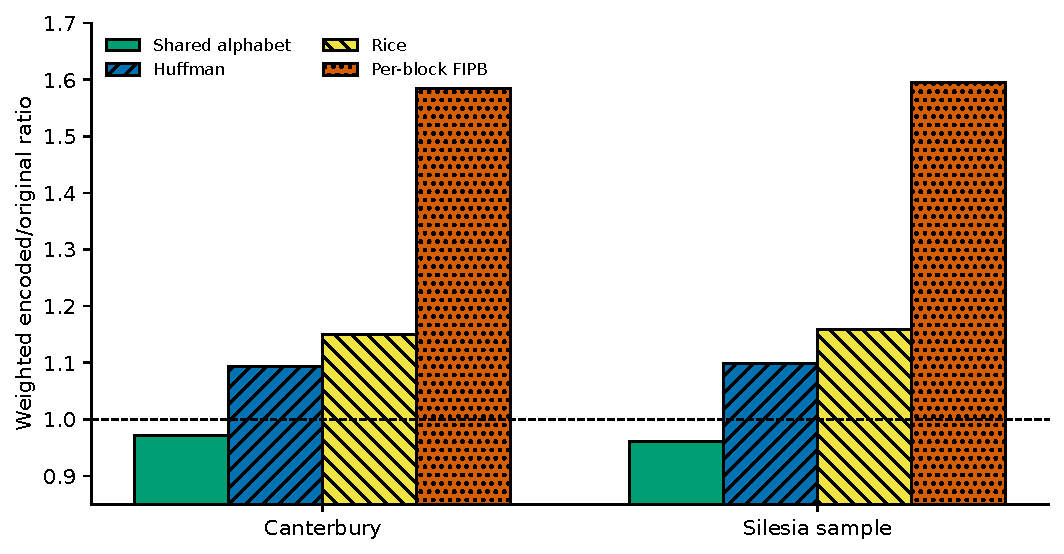
\includegraphics[width=0.72\textwidth]{artwork/Figure_3_Gap_Coding_Comparison.pdf}
\caption{Weighted size comparison on identical 256-byte Fibonacci gap streams.
The Silesia values use fixed 64\,KiB prefixes; full-corpus results appear in
Table~\ref{tab:corpus}.}
\label{fig:gap-coding}
\end{figure*}

On complete files, the shared stream compresses \texttt{ptt5} to 0.8424,
\texttt{mozilla} to 0.9938, and \texttt{mr} to 0.7732. The apparent gain on
the 64\,KiB \texttt{ooffice} prefix does not persist on the complete file.
The \texttt{mozilla} ratio likewise changes from 0.7672 on its fixed prefix to
0.9938 on the complete file, an absolute increase of 0.2266. This change
indicates that the prefix has a substantially higher concentration of
favorable structure than the remaining file. Other files select the stream-level
raw branch. These cases justify restricting prefix results to sensitivity
analysis and basing corpus claims on complete inputs.

\subsection{Universal-code comparison}

Replacing fixed identifiers with a standard universal code does not remove
the limitation. At a 256-byte block size on Canterbury, the optimistic
payload-only ratios are 0.9439 for delimiter-free fixed binary gap values,
1.1612 for oracle Rice coding, 1.5007 for Elias gamma, 1.5152 for Fibonacci
universal coding, 1.7612 for Elias delta, and 3.0960 for LEB128. The same
ordering is observed on fixed Silesia prefixes. The fixed-binary figure is not a
complete decodable stream because it omits delimiters; it serves only to
isolate the intrinsic gap magnitudes.

\subsection{Corpus-level compression}

Table~\ref{tab:block-sensitivity} reports the full-corpus block-size
sensitivity. Canterbury is smallest at 32 bytes, whereas Silesia is smallest
at 256 bytes. The difference follows from two competing costs. Short blocks
make sparse local patterns easier to isolate but create more block records;
long blocks amortize those records but usually contain more Zeckendorf terms.
No tested size makes the method broadly applicable. Only one Canterbury file
compresses at every size, and Silesia has one compressed file through
128 bytes and two at 256 bytes.

\begin{table*}[t]
\caption{Complete shared-stream sensitivity to block size.}
\label{tab:block-sensitivity}
\centering
\begin{tabular}{rrrrrrr}
\toprule
& \multicolumn{3}{c}{Canterbury} & \multicolumn{3}{c}{Silesia}\\
\cmidrule(lr){2-4}\cmidrule(lr){5-7}
Block & Ratio & Files $<1$ & Shared (\%) & Ratio & Files $<1$ & Shared (\%)\\
\midrule
16  & 0.9274 & 1 & 12.956 & 0.9978 & 1 & 3.084\\
32  & 0.9215 & 1 & 11.353 & 0.9930 & 1 & 2.745\\
64  & 0.9354 & 1 &  9.136 & 0.9905 & 1 & 2.497\\
128 & 0.9593 & 1 &  6.100 & 0.9900 & 1 & 2.227\\
256 & 0.9713 & 1 &  3.750 & 0.9878 & 2 & 1.938\\
\bottomrule
\end{tabular}
\tablenote{Ratios include all stream and block fields. ``Shared'' is the
fraction of blocks that select the gap representation.}
\end{table*}

The remaining cross-method tables use 256 bytes as a common reference rather
than selecting a different size for each corpus. At that setting, FISA reaches
0.9713 on Canterbury and 0.9878 on Silesia. The complete \texttt{ooffice}
file selects the raw-stream branch, showing why prefix results cannot be
extrapolated to a full file.

\begin{table*}[t]
\caption{Complete-corpus comparison at the common 256-byte FISA setting.}
\label{tab:corpus}
\centering
\begin{tabular}{lrrr}
\toprule
Corpus & Files & Weighted shared & Best weighted modern\\
\midrule
Canterbury & 11 & 0.9713 & 0.1746\\
Silesia complete & 12 & 0.9878 & 0.2302\\
enwik8 & 1 & 1.0000001 & 0.2483\\
\bottomrule
\end{tabular}
\tablenote{The modern column selects the smallest tested codec for each file.
On enwik8, FISA selects raw storage and adds 10 framing bytes to the
100,000,000-byte input.}
\end{table*}

Modern codecs win every paired file comparison. These comparisons define the
scope of the shared representation: it is a conditional transform rather than
a general-purpose codec.

The modern-codec oracle wins all 11 Canterbury comparisons and all 12 Silesia
comparisons. The median FISA-to-oracle ratio factors are 3.92 and 4.23.
These win counts establish the direction of the measured result on the
evaluated files; the small corpus counts do not support broad distributional
inference.

For context, full-corpus weighted ratios on Canterbury are 0.1746 for Brotli,
0.1751 for LZMA, 0.1819 for PPMd, 0.1837 for Zstandard, 0.1931 for bzip2, and
0.2589 for zlib. On full Silesia, the corresponding ratios are 0.2375,
0.2302, 0.2367, 0.2497, 0.2572, and 0.3192.

Table~\ref{tab:notable-files} reports the complete-file cases discussed in the
text. It includes the three files that compress at 256 bytes, the
\texttt{ooffice} prefix counterexample, and \texttt{x-ray} as a representative
raw-fallback file.

\begin{table}[t]
\caption{Selected complete-file FISA outcomes at 256-byte blocks.}
\label{tab:notable-files}
\centering
\begin{tabular}{llrr}
\toprule
Corpus & File & Ratio & Shared blocks\\
\midrule
Canterbury & \texttt{ptt5}    & 0.842370 & 411\\
Silesia    & \texttt{mozilla} & 0.993760 & 5,309\\
Silesia    & \texttt{mr}      & 0.773155 & 9,652\\
Silesia    & \texttt{ooffice} & 1.000002 & 122\\
Silesia    & \texttt{x-ray}   & 1.000001 & 0\\
\bottomrule
\end{tabular}
\tablenote{A file may contain locally selected shared blocks yet still select
the raw stream after complete stream-level accounting.}
\end{table}

\subsection{Sparse-structure controls}

Zero dominance alone is not a sufficient application criterion. In a
controlled 1\,MiB corpus with independently positioned nonzero bytes, FISA
has ratio 0.8650 at 1\% density and selects raw storage from 5\% density
upward. At 1\% density, the measured general-purpose ratios range from 0.0217
for PPMd to 0.0327 for zlib.

Figure~\ref{fig:structural-controls} compares FISA with two complete, exactly
decodable controls after the same block-size sweep. The bitmap method stores
one presence bit per block and copies nonzero blocks. The trim method stores
the leading-zero count and the middle span of every block. Both controls attain
a smaller corpus ratio than FISA.

\begin{figure*}[t]
\centering
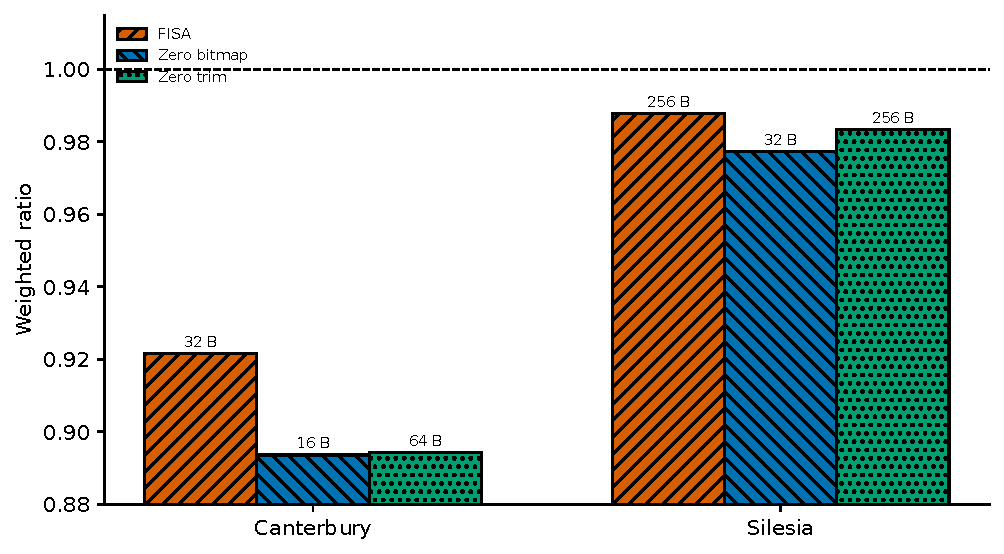
\includegraphics[width=0.68\textwidth]{artwork/Figure_4_Structural_Controls.pdf}
\caption{Structural controls at their best tested block sizes. A ratio below
one denotes compression; lower values indicate smaller complete streams.
Labels above the bars give the selected block size in bytes.}
\label{fig:structural-controls}
\end{figure*}

The matched sweeps strengthen the structural explanation. On Canterbury, the
best bitmap and trim streams save about 2.8 percentage points beyond the best
FISA stream. On Silesia, the best bitmap saves about 1.0 percentage point.
Block-level zero structure accounts for the favorable cases with less
machinery than Fibonacci decomposition.
Even these controls remain far above the modern-codec oracle: their best
weighted ratios are 0.8936 and 0.8942 on Canterbury, compared with 0.1746,
and 0.9774 and 0.9833 on Silesia, compared with 0.2302.
They do outperform byte RLE, whose weighted ratios are 1.5321 and 1.7288, but
not zlib at 0.2589 and 0.3192. The controls therefore isolate zero structure
more economically than FISA without approaching a dictionary codec.

\subsection{Monotone integer sequences and enwik8}

Elias--Fano is evaluated only on its intended domain: strictly increasing
integer sequences. On five deterministic 100,000-value datasets it requires
2.00, 3.00, 4.25, 3.52, and 18.53 bits per integer for dense, geometric
($p=0.5$), geometric ($p=0.2$), posting-like, and quadratic sequences.
Complete gap Rice coding ranges from 1.00 to 18.03 bits per integer, while
complete gap Huffman is best on the posting-like sequence at 1.82 bits per
integer. These results show that no single integer representation dominates:
the source distribution and monotonicity determine the appropriate code.

On the 100,000,000-byte enwik8 corpus, complete ratios are 0.2483 for PPMd,
0.2487 for LZMA, 0.2694 for Zstandard, 0.2705 for Brotli, 0.2901 for bzip2,
0.3648 for zlib, and 1.0000001 for compiled FISA. FISA writes
100,000,010 bytes: the raw input plus 10 bytes of stream framing. This
benchmark confirms the fallback behaviour on an unfavorable large input.

\subsection{Entropy and context}

Mean empirical zero-order entropy is 4.4051 bits/byte on Canterbury and 5.0498
bits/byte on fixed Silesia prefixes. The corresponding first-order conditional
values are 3.0015 and 3.4052 bits/byte. The reductions of 1.4036 and 1.6446
bits/byte indicate substantial sequential dependence. The current block
integer transform does not explicitly model this dependence, whereas
dictionary and context-based codecs can exploit it.

\section{Discussion}
\label{sec:discussion}

\subsection{Why compression remained rare}

A favorable block needs a sparse Zeckendorf decomposition and repeated gap
values. Even then, the saved bits must cover its record and a share of the
file-level alphabet. Most text and binary blocks already fail at sparsity.
Zero-dominated blocks sometimes pass, but the bitmap and trim controls encode
the same structure with less machinery.

The \texttt{mozilla} file gives a concrete warning. Its first 64\,KiB produced
a ratio of 0.7672, which looked useful. The complete file reached 0.9938.
The prefix happened to contain much more favorable structure than the rest of
the input. A result based on that prefix alone would have overstated the
method's practical range.

Changing the block size did not rescue the representation. Short blocks
isolate local zero regions but create more records. Long blocks reduce that
record cost and select more Fibonacci terms. Canterbury favored 32 bytes;
Silesia favored 256. At either optimum, almost every file still used the raw
branch.

\subsection{What byte-level accounting revealed}

The gap statistic and the serialized stream answer different questions.
Several delimiter-free gap lists are shorter than raw binary, but they do not
identify symbol boundaries and they carry no alphabet. Equations
\eqref{eq:exact-shared-condition} and \eqref{eq:k-threshold} put those omitted
bytes back into the comparison. They show where a positional transform stops
saving space once its model and records are present.

\subsection{Comparison with established coding methods}

FISA converts each block to one large integer. The mapping is reversible, so
it does not destroy information, but the gap model no longer exposes byte
adjacency directly. The measured first-order reductions of 1.4036 and 1.6446
bits per byte quantify dependence available to sequence models and absent
from FISA's blockwise identifier model. This modelling choice is consistent
with the median 3.92--4.23 size-factor gap to the modern-codec oracle.
Fibonacci universal coding solves a
different problem because it self-delimits positive integers; FISA instead
stores gaps under a shared alphabet. Binary-position gaps are the closer
structural comparison. Their result makes clear that the favorable integer
count is not a Fibonacci effect.

\subsection{Limitations}

The Python implementation remains a clarity-oriented reference. A compiled
Java implementation with cached Fibonacci tables evaluates all 211.9\,MB of
Silesia and the 100\,MB enwik8 file. Runtime measurements are retained in the
reproducibility package, but no cross-codec speed claim is made because the
evaluated baselines use different runtimes and bindings.
Within the same Java implementation, the asymmetry is substantial:
Canterbury encodes at 0.758\,MiB/s and decodes at 113.3\,MiB/s, while Silesia
encodes at 1.423\,MiB/s and decodes at 1305.9\,MiB/s. These are approximately
149-fold and 918-fold differences. Encoding performs large-integer
Zeckendorf decomposition for every candidate block. Decoding is dominated by
copying raw data because 96.25\% of Canterbury blocks and 98.06\% of Silesia
blocks do not use the shared representation at the 256-byte setting.

The format uses one stream-level alphabet and fixed-width
identifiers. Hierarchical alphabets, canonical entropy codes over the shared
identifier stream, or context models may further reduce overhead, but they
would require separate specification and measurement. The integer sweep covers
the range up to $10^7$; larger block integers are sampled through the corpus
experiments rather than exhaustively enumerated.

The normative format uses big-endian block integers. A reversible
little-endian sensitivity check at 256 bytes gives 0.9712 instead of 0.9713
on Canterbury and 0.9580 instead of 0.9608 on fixed Silesia prefixes. Byte
order changes which boundary zeros become high-order integer zeros, but the
measured differences do not alter the conclusion.

\subsection{Implications}

The evidence does not support further optimization of FISA as a
general-purpose codec. A more promising continuation is an adaptive sparse
block representation that selects directly among zero bitmaps, boundary
trimming, binary positions, and raw storage. The cost equations and
decode-after-encode checks remain useful for evaluating such a system.

\section{Conclusion}
\label{sec:conclusion}

We asked whether Fibonacci index gaps remain smaller after a decoder's full
input is serialized. Usually, they do not. FISA is reversible, and its best
weighted ratios are 0.9215 on Canterbury and 0.9878 on Silesia, but only one
and two files compress. Every established codec wins its paired comparisons.

The controls explain the few positive cases. Binary set-bit positions improve
the integer-level statistic without using Fibonacci. On complete files,
zero-block bitmaps and boundary trimming are smaller than FISA. The main
result is a boundary, not a new general-purpose codec: sparse index gaps can
look compact while their alphabet and records erase the saving. Future work
should start from the observed zero structure and compare its serialized cost
directly, before assigning the gain to a number system.

\section*{Acknowledgements}

This work was supported by the authors' institutions. No external financial
support was received.

\printcredits

\section*{Declarations}

\noindent\textbf{Ethics approval.}
This study does not involve human participants, animals, personal data, or
clinical interventions. It uses publicly available benchmark corpora,
synthetic data, and offline computational experiments.

\medskip
\noindent\textbf{Competing interests.}
The authors declare that they have no known competing financial interests or
personal relationships that could have appeared to influence the work
reported in this paper.

\medskip
\noindent\textbf{Funding.}
This research received no external funding.

\medskip
\noindent\textbf{Data availability.}
The Canterbury corpus, Silesia corpus, and enwik8 benchmark are publicly
available from their original distributors under their applicable terms.
The fixed samples, synthetic-data generators, aggregate results, and per-file
evaluation artefacts accompany the reproducibility package.

\medskip
\noindent\textbf{Code availability.}
The reproducibility package contains the reference implementation, tests,
experiment configurations, evaluation scripts, machine-readable result
tables, figure-generation code, and exact random seeds. It is publicly
available at
\url{https://github.com/EkodeckStephane/fibonacci-index-gap-coding}.
An archival DOI will be added when the repository is deposited.

\appendix

\section{Container fields}
\label{app:format}

Table~\ref{tab:container-fields} lists every serialized field in FISA 1.0.

\begin{table}[H]
\caption{FISA 1.0 shared-stream fields.}
\label{tab:container-fields}
\centering
\resizebox{\columnwidth}{!}{%
\begin{tabular}{lll}
\toprule
Scope & Field & Encoding\\
\midrule
Stream & Magic & ASCII \texttt{FISA}\\
Stream & Format identifier & One byte, value 1\\
Stream & Stream mode & One byte: 0 raw, 1 shared\\
Stream & Original byte length & Variable-length integer\\
\midrule
Raw stream & Payload & Exactly the original byte length\\
\midrule
Shared stream & Nominal block size & Variable-length integer\\
Shared stream & Number of blocks & Variable-length integer\\
Shared stream & Alphabet size & Variable-length integer\\
Shared stream & Symbol width & One byte\\
Shared stream & Alphabet values & Variable-length integers\\
\midrule
Block & Mode & One byte: 0 raw, 1 shared identifiers\\
Block & Original block length & Variable-length integer\\
Block & Payload length & Variable-length integer\\
Block & Payload & Declared number of bytes\\
\midrule
Shared payload & Symbol count & Variable-length integer\\
Shared payload & Packed length & Variable-length integer\\
Shared payload & Symbol identifiers & Fixed-width, MSB first\\
\bottomrule
\end{tabular}
}
\tablenote{All variable-length integers use unsigned LEB128.}
\end{table}

\subsection{Structural grammar}

The following ABNF-like grammar uses \texttt{uvarint} for the shortest unsigned
LEB128 form and \texttt{byte\{n\}} for exactly $n$ bytes.
\begin{verbatim}
stream        = "FISA" version stream-mode
                original-length body
body          = raw-stream / shared-stream
version       = %x01
stream-mode   = %x00 / %x01
raw-stream    = byte{original-length}
shared-stream = block-size block-count
                alphabet-size width alphabet block-list
alphabet      = uvarint{alphabet-size}
block-list    = block{block-count}
block         = block-mode block-length payload-length
                block-payload
block-mode    = %x00 / %x01
block-payload = raw-payload / shared-body
raw-payload   = byte{payload-length}
shared-body   = symbol-count packed-length
                byte{packed-length}
\end{verbatim}

The selected branch is determined by \texttt{stream-mode}. In shared mode,
the \texttt{block-mode} field determines the conditional alternative:
mode 1 requires \texttt{block-payload = shared-body}, whereas mode 0 requires
\texttt{block-payload = raw-payload} and
\texttt{payload-length = block-length}. For mode 1, the bytes consumed by
\texttt{shared-body} must equal \texttt{payload-length}.

\subsection{Degenerate cases and mandatory errors}

An empty input has original length zero, zero blocks, and is represented by
the raw stream branch. A zero-valued nonempty block has an empty gap sequence;
its declared block length preserves all leading zero bytes. The decoder must
reject an unknown magic, format identifier, stream mode, or block mode;
truncated or unreasonably long length fields; zero block size in shared mode;
symbol identifiers outside the alphabet; packed lengths inconsistent with
symbol count and width; reconstructed integers exceeding their block length;
incorrect final length; and trailing bytes after the declared stream.

\section{Reproducibility checklist}
\label{app:reproducibility}

\begin{itemize}
\item Python 3.13.5 and a Java 8-compatible compiled implementation; package
versions are pinned in the experiment dependency manifest.
\item Synthetic seed: 20260608.
\item Exact decode-after-encode verification for every measured FISA stream.
\item Final automated test result: 10,119 passed.
\item Bootstrap iterations: 10,000.
\item All output sizes include stream and block framing for complete-codec
results. Payload-only universal-code comparisons are labeled explicitly.
\end{itemize}

\section*{Declaration of generative AI and AI-assisted technologies in the
manuscript preparation process}

During the preparation of this work, the authors used the OpenAI Codex coding
agent to assist
with source-code editing, experiment orchestration, language editing,
formatting, and consistency checks. After using this service, the authors
reviewed and edited the outputs, reran the reported workflows, verified the
results against the source data, and take full responsibility for the content
of the publication.

\clearpage
\bibliographystyle{cas-model1-num-names}
\bibliography{cas-refs}

\end{document}
